\documentclass{article}
\usepackage{graphicx}
\usepackage{caption}
\usepackage[dblblindworkshop]{neurips_2026}
\workshoptitle{TAE (Trust-AI-Eval): Can We Trust AI Evaluation?}
\usepackage[utf8]{inputenc}
\usepackage[T1]{fontenc}
\usepackage{hyperref}
\usepackage{url}
\usepackage{booktabs}
\usepackage{amsfonts}
\usepackage{amssymb}
\usepackage{nicefrac}
\usepackage{microtype}
\usepackage{xcolor}
\usepackage{float}
\usepackage{calc}
\usepackage{amsmath}
\usepackage{longtable}
\usepackage{array}

\providecommand{\tightlist}{%
  \setlength{\itemsep}{0pt}\setlength{\parskip}{0pt}}

\makeatletter
\def\maxwidth{\ifdim\Gin@nat@width>\linewidth\linewidth\else\Gin@nat@width\fi}
\def\maxheight{\ifdim\Gin@nat@height>0.82\textheight 0.82\textheight\else\Gin@nat@height\fi}
\makeatother
\setkeys{Gin}{width=\maxwidth,height=\maxheight,keepaspectratio}

\hypersetup{
  colorlinks=true,
  linkcolor=black,
  citecolor=black,
  urlcolor=black,
  pdfauthor={Anonymous},
  pdftitle={ECHO: Diagnosing Spatial Cue Access in Audio-Language Models},
  pdfsubject={Anonymous workshop submission},
  pdfcreator={LaTeX}
}

\title{ECHO: Diagnosing Spatial Cue Access in Audio-Language Models}
\author{Anonymous Author(s)}

\begin{document}
\maketitle
\raggedbottom

\begin{abstract}
Stereo localization requires an audio-language model---a system that accepts audio and answers in language---to recover spatial evidence from left and right signals and use it to infer direction. Traditional end-to-end accuracy reports only whether the final direction is correct, hiding whether a model failed to obtain the spatial cue or failed to use it. We introduce ECHO (Explicit Cue versus Heard Observation), a paired diagnostic framework, and StereoMusicQA, a benchmark built from real instrument recordings rendered at known positions. Together, they test whether a model can use a spatial cue that it fails to obtain through audio. Each of 1,045 test items has two views: \emph{cue-text} provides the measured left-right level difference and conversion equation; \emph{audio-only} provides labeled channels and requires the model to obtain a useful relationship from audio. Because cue-text also supplies the rule, this comparison measures the practical advantage of a written cue and rule, not the effect of one internal layer. For Qwen2-Audio, Gemini Flash-Lite, and GPT-audio, cue-text left/center/right accuracy is 71.9\%, 93.6\%, and 90.4\% compared with 28.5\%, 36.6\%, and 42.0\% audio-only. These 43.3--57.0 percentage-point gains remain positive when complete source tracks are resampled. Furthermore, a model can identify the correct side yet still predict an inaccurate angle: cue-text within-\(5^\circ\) accuracy ranges from 0.4\% to 80.7\%, and written-calculation faithfulness ranges from 0.4\% to 77.8\%. ECHO therefore shows why spatial evaluation should separately test evidence access, cue use, and whether a stated calculation follows from the cue.

\end{abstract}

\section{Introduction}
\label{sec:introduction}

Spatial information matters whenever an audio system must do more than just name a sound. A music assistant cannot reliably follow a set of instructions like "move the violin towards the center", unless it knows the position of the violin. An accessibility system may recognize a car yet fail to say whether it is on the listener's left or right. A useful audio assistant therefore needs both semantic information---\emph{what} produced the sound---and spatial information---\emph{where} the sound is.

Stereo audio contains a left channel and a right channel. When a source is placed to one side, the two channels usually differ. In StereoMusicQA, position is represented by a level difference: a leftward source has more amplitude in the left channel, and a rightward source has more amplitude in the right channel. This measured difference is called the inter-channel level difference, or ILD. ILD is a \emph{spatial cue}: a measurable piece of evidence about position. It is reported in decibels (dB); its sign indicates the louder side, and its magnitude can be converted to an angle using a panning equation. Panning is the studio process of placing a mono sound toward the left or right by changing its level in the two channels.

Recent benchmarks show that general-purpose audio-language models often struggle with basic physical properties such as loudness, pitch, and direction even when they can describe higher-level audio content \citep{gong2024avodyssey,sun2026sonicbench}. Purpose-built systems such as BAT and OWL add spatially specialized encoders or supervision \citep{zheng2024bat,biswas2025owl}, but a final localization score still does not reveal whether an error began when the model accessed the spatial evidence or when it used that evidence.

When an audio-language model is asked to localize a stereo source, it faces a two-stage problem. First, the model must compare the left and right audio and obtain a useful cue such as ILD. Second, it must use that cue to decide the side or calculate the angle. We call these stages \emph{cue access} and \emph{cue use}. If a model gives the wrong final answer, an ordinary benchmark cannot tell whether it failed at the first stage, the second stage, or both. That distinction matters because the repairs are different: arithmetic training cannot recover evidence that never reaches the language model, while better early audio processing does not guarantee correct reasoning from an available cue. A single score therefore does not show whether to improve audio processing, channel comparison, or later numerical reasoning.

\emph{Explicit Cue versus Heard Observation} (ECHO) is designed to reveal which stage fails. StereoMusicQA supplies controlled test items built from real instrument recordings placed at known angles with a reversible panning rule. Here, localization means identifying whether a source is left, centered, or right and estimating its angle. We ask:

\begin{quote}
    When this localization task and its correct answer stay fixed, how much does performance change when the spatial cue and conversion rule are written explicitly rather than left for the model to recover and apply from audio?
\end{quote}

For a concrete example, consider one violin placed left of center. The cue-text version gives the model mono (single-channel) audio plus a statement such as "the left channel is 6 dB louder" and provides the conversion equation. The audio-only version gives the two rendered channels but does not state their level difference. Both versions ask for the same side and angle, and both have the same correct answer. If a model succeeds only when the 6 dB difference is written down, it has shown some ability to use that evidence under a supplied rule but has not made the same evidence reliably usable from audio. We call this operational within-item contrast the \emph{cue-access gap}.

Across 1,045 matched items, writing the cue and rule explicitly raises left/center/right accuracy by 43.3-57.0 percentage points for all three tested models, while every audio-only estimate remains below the most-common-label baseline. Correct side predictions still do not guarantee accurate angles or faithful written calculations. Together, these results show that one end-to-end score can hide different failures that require different remedies.

\begin{figure}[!htbp]
\centering
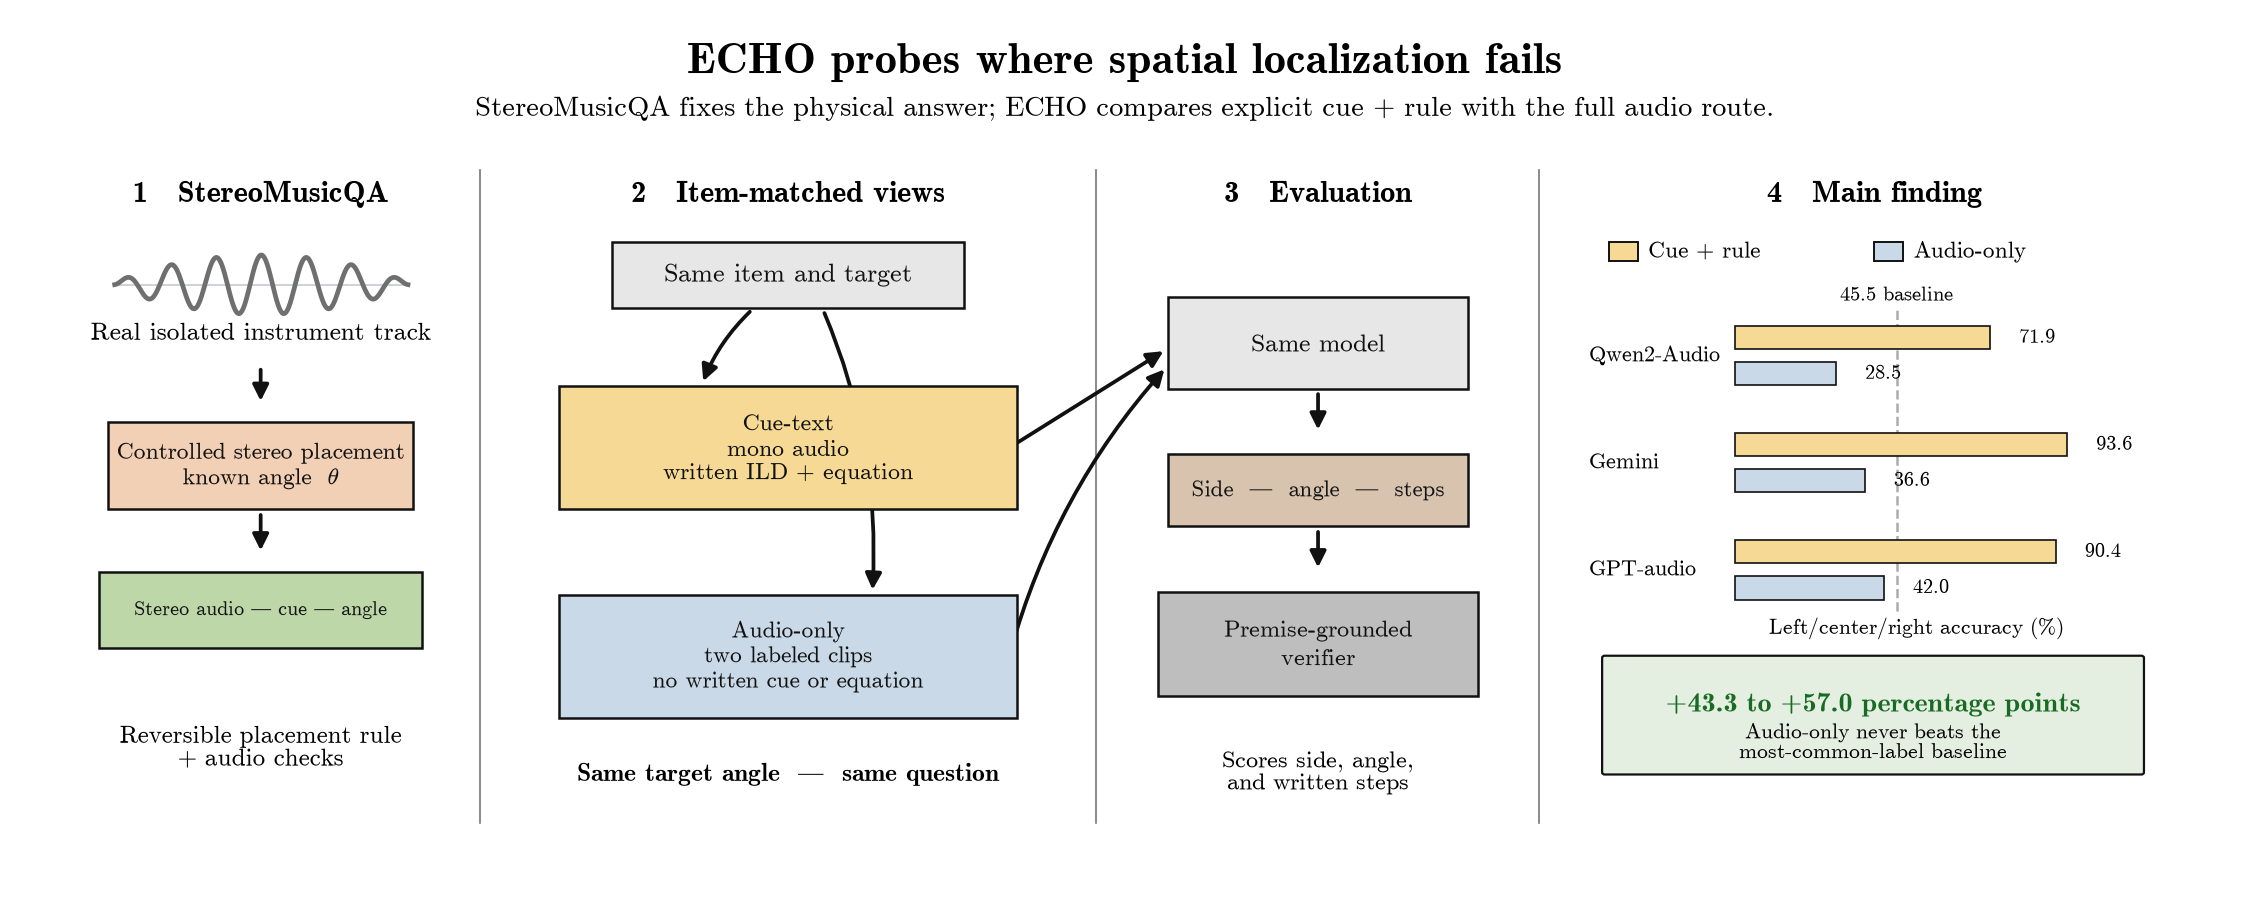
\includegraphics[width=\linewidth]{figures/fig0_framework_and_benchmark.png}
\caption{StereoMusicQA places a real instrument recording at a known angle. ECHO asks the same question with the cue and rule written in text or with the relationship available only through audio; the answer, model, and scorer stay fixed. Cue-text improves left/center/right accuracy by 43.3--57.0 percentage points, while every audio-only result remains below the most-common-label baseline.}

\label{fig:framework}
\end{figure}

In summary, our contributions are:
\footnote{\href{https://anonymous.4open.science/r/ECHO-FC6D/}{Anonymous code and artifacts} include benchmark manifests, prompts, model completions, and evaluation scripts. URMP source audio is not redistributed and must be obtained from its original distribution.}

\begin{enumerate}
\def\labelenumi{\arabic{enumi}.}
\tightlist
\item
    \textbf{A framework and benchmark.} ECHO compares the same item through the full audio path and best-case explicit cue use. StereoMusicQA uses real recordings, controlled positions, and a reversible rule that makes the cue and answer recomputable.
\item
    \textbf{Evidence of a cue-access gap.} On the same 1,045 items, three general-purpose audio language models are 43.3--57.0 percentage points more accurate at classifying left, center, or right when the cue and rule are explicit. Confidence intervals obtained by resampling complete source tracks exclude zero for each model.
\item
    \textbf{Stage-specific scoring.} ECHO separately measures coarse left/center/right decisions, numerical angle accuracy, and whether each written calculation follows from the cue stated in the response.
\end{enumerate}

\section{Related Works}

\paragraph{Physical audio evaluation}
AV-Odyssey shows that models combining audio and vision can fail basic loudness and pitch comparisons \citep{gong2024avodyssey}. SonicBench evaluates twelve measurable audio properties and reports broad difficulty, including direction \citep{sun2026sonicbench}. Some properties remain predictable from early audio features even when final answers fail. SpeechR finds a related gap in speech: recognizing words does not guarantee reasoning correctly about them \citep{yang2025speechr}. ECHO narrows this question to left-right position and changes whether the cue and rule are written explicitly or must be obtained and used through audio.

\paragraph{Purpose-built spatial audio-language systems}
BAT combines a specialized spatial audio encoder with a language model \citep{zheng2024bat}; SALM separates semantic and spatial information \citep{hu2025salm}; OWL adds geometric supervision \citep{biswas2025owl}; and Dual-BEATs uses one encoder per channel and reports that training noise can help preserve channel differences through internal normalization \citep{lin2026dualbeats}. These systems ask how to build better spatial models. ECHO instead audits where an existing general-purpose system may fail.

\paragraph{Evaluation validity.}
Related problems occur beyond audio. Vision-language models can describe scenes while failing simple geometry \citep{rahmanzadehgervi2024blind}; models can score well by learning shortcuts rather than the intended rule \citep{geirhos2020shortcut}; and plausible step-by-step explanations need not faithfully reflect the basis of an answer \citep{turpin2023unfaithful}. ECHO tests these concerns through item-matched conditions, an off-grid stress test, and a verifier that recomputes arithmetic from the model's stated cue. Table~\ref{tab:benchmark-comparison} compares the experimental designs of nearby benchmarks; their scores are not placed on one leaderboard because their tasks and labels differ.

\section{ECHO and StereoMusicQA}
\label{sec:methods}

ECHO is an evaluation framework for locating where failure may arise inside a spatial-audio question-answering pipeline. StereoMusicQA is the benchmark that makes this comparison possible. The distinction is:
\begin{itemize}
\tightlist
\item
    \textbf{StereoMusicQA creates the problem.} It produces stereo audio with a known source angle, a measurable left-right cue, and a correct answer that can be computed.
\item
    \textbf{ECHO creates the comparison.} It asks the same question once with that cue and its conversion rule stated in text, and once with the relevant relationship available only in the audio channels.
\end{itemize}

The complete evaluation follows five steps. (1) Create a spatial item with known ground truth. (2) Make matched cue-text and audio-only versions. (3) Collect one answer from each model in each condition. (4) Score the reported side and angle, and check any written calculation. (5) Compare the two answers from the same item. The following subsections explain each step and the assumptions behind them.

\subsection{StereoMusicQA construction}

StereoMusicQA begins with the University of Rochester Multi-Modal Music Performance Dataset (URMP) \citep{li2019urmp}. URMP contains 149 isolated instrument tracks from 44 classical chamber pieces. An isolated track is a recording of one performer's part without the other instruments. Each track is mono, meaning that it has one channel and therefore no original left-right position. URMP supplies the real music sound; we create the spatial position ourselves.

We place each mono recording at a chosen horizontal angle and render a new left and right channel. Positive angles mean left, zero means center, and negative angles mean right. The main study uses 1,045 held-out single-source items made from 19 tracks in six pieces. We split by complete musical piece, so a performance used for testing never appears in training.

Each held-out track is rendered at eleven angles from \(-25^\circ\) to \(+25^\circ\) under an unchanged condition and four common audio transformations. Because these are repeated versions of 19 recordings, Section~\ref{sec:uncertainty} treats them as related observations rather than 1,045 independent sources. Appendix~\ref{sec:appendix-construction} gives full construction details.

For the main experiment, we use amplitude panning. This is the familiar studio operation that moves a mono signal left or right by changing its level in the two output channels. The panning law uses virtual speaker anchors at \(+30^\circ\) on the left and \(-30^\circ\) on the right; the tested source angles stay within \(\pm25^\circ\). The interchannel level difference is defined as \(\mathrm{ILD}=20\log_{10}(L/R)\), where \(L\) and \(R\) are the left- and right-channel amplitudes. We call the horizontal source angle the azimuth and denote it by \(\theta\). Thus positive ILD and positive \(\theta\) indicate left, while negative values indicate right. If \(r=L/R\), then

\[
r = 10^{\mathrm{ILD}/20}, \qquad
d = \frac{r-1}{r+1}, \qquad
\theta = \arctan\!\left(d\tan 30^\circ\right).
\]

This equation makes the benchmark checkable in both directions. We know the angle used to create the audio, and we can measure the finished left and right channels, recover ILD, and obtain the same angle. Items that fail this check are rejected.

This design is controlled studio panning, not a simulation of natural human hearing, which also depends on the listener's anatomy, room, frequency, elevation, and distance. We use the simpler case because it gives an exact link among waveform, cue, and answer.

\subsection{Two conditions for one localization problem}

Each item is presented in two matched ways:

\begin{itemize}
\tightlist
\item
  \textbf{Cue-text condition.} The model receives mono audio, so it still hears the musical content, but the prompt explicitly states the measured ILD, identifies the louder channel, and gives the panning equation. The model must use the supplied cue by following the provided rule.
\item
  \textbf{Audio-only condition.} The model receives the left and right channels as two separately labeled audio clips. The prompt does not state ILD or the panning equation. The model must compare the clips and obtain a useful spatial relationship through its audio interface.
\end{itemize}

The source rendering, planted position, question, correct answer, model, and scoring rule remain fixed. The information supplied to the model is not otherwise identical: cue-text provides both the measured cue and the conversion rule, whereas audio-only provides neither. The paired gap therefore measures the practical advantage of explicit symbolic access over the full audio route. It does not cleanly separate extracting the cue from knowing or applying the conversion rule. An audio-plus-rule condition would be needed to isolate that distinction more tightly.

There is also an important delivery limitation: Qwen2-Audio's audio input component accepts mono audio, so we cannot pass one native stereo file consistently across all systems. Separate labeled clips preserve left and right identity, but the model must still compare two audio sequences. Thus ECHO measures the complete practical access path, including audio ingestion, cross-channel comparison, alignment with the language model, and answer generation. This comparison alone cannot identify one responsible internal layer.

\subsection{Models}

We test Qwen2-Audio-7b-Instruct locally \citep{chu2024qwen2audio} and Gemini Flash-Lite and GPT-audio through their hosted application programming interfaces (APIs). Each model receives all 1,045 items in both conditions, with instructions but no solved examples, and produces one answer per item. Only Qwen2-Audio exposes the internal features needed for probing and fine-tuning. Appendix~\ref{sec:appendix-repro} records exact settings and the limitations of changing hosted services.

\subsection{Scoring and checking written calculations}

We score three outcomes. \textbf{Left/center/right accuracy} is the percentage assigned the correct position label. Table~\ref{tab:complete-results} also reports class-balanced measures so a frequent default answer is not rewarded. \textbf{Angle accuracy} asks whether the prediction is within \(5^\circ\) of the planted angle; mean absolute error reports the average error size. \textbf{Stated-derivation faithfulness} asks whether the visible calculation follows mathematically from the cue in the response.

Unanswered items count as wrong. In cue-text answers, the final signed angle determines side because the prompt defines positive as left and negative as right. In audio-only answers, we score the explicit word "left", "center", or "right" because that prompt does not introduce a numeric sign convention. Every model uses the same extraction rule within a condition.

We implement a deterministic \emph{verifier}: a program that parses the model's written steps and recomputes them from the stated premise rather than checking only the final answer. If the model writes \(r=10^{x/20}=y\), it recomputes \(y\) from the stated \(x\) before checking the later angle. This catches a response that copies the cue but silently calculates with a memorized value. We call the check \emph{premise-grounded} because it begins with the premise stated in the answer. Appendix~\ref{sec:appendix-offgrid} documents the off-grid audit that motivated this stricter check: a response can resemble a solved equation using a value that does not follow from its own first line.

\subsection{Uncertainty and dependence}
\label{sec:uncertainty}

The 1,045 items are not 1,045 unrelated recordings. They reuse 19 source tracks at different angles and with different processing. Treating every render as independent would make the result look more certain than it is. We therefore resample complete tracks, rather than individual items, 20,000 times while keeping each item's two conditions paired. The middle 95\% of the resulting differences form the confidence interval. A stricter check groups the tracks by their six musical pieces; all paired intervals still exclude zero. Appendix~\ref{sec:appendix-stats} gives the procedure and cautions that six pieces provide limited precision.

\section{Results}
\label{sec:results}

\subsection{Explicit cues and rules reveal a large performance gap}

As Figure~\ref{fig:main-gap} shows, left/center/right accuracy is higher for every model when the level difference and conversion rule are written in the prompt than when the model must obtain and use a relationship from audio.

\begin{figure}[H]
\centering
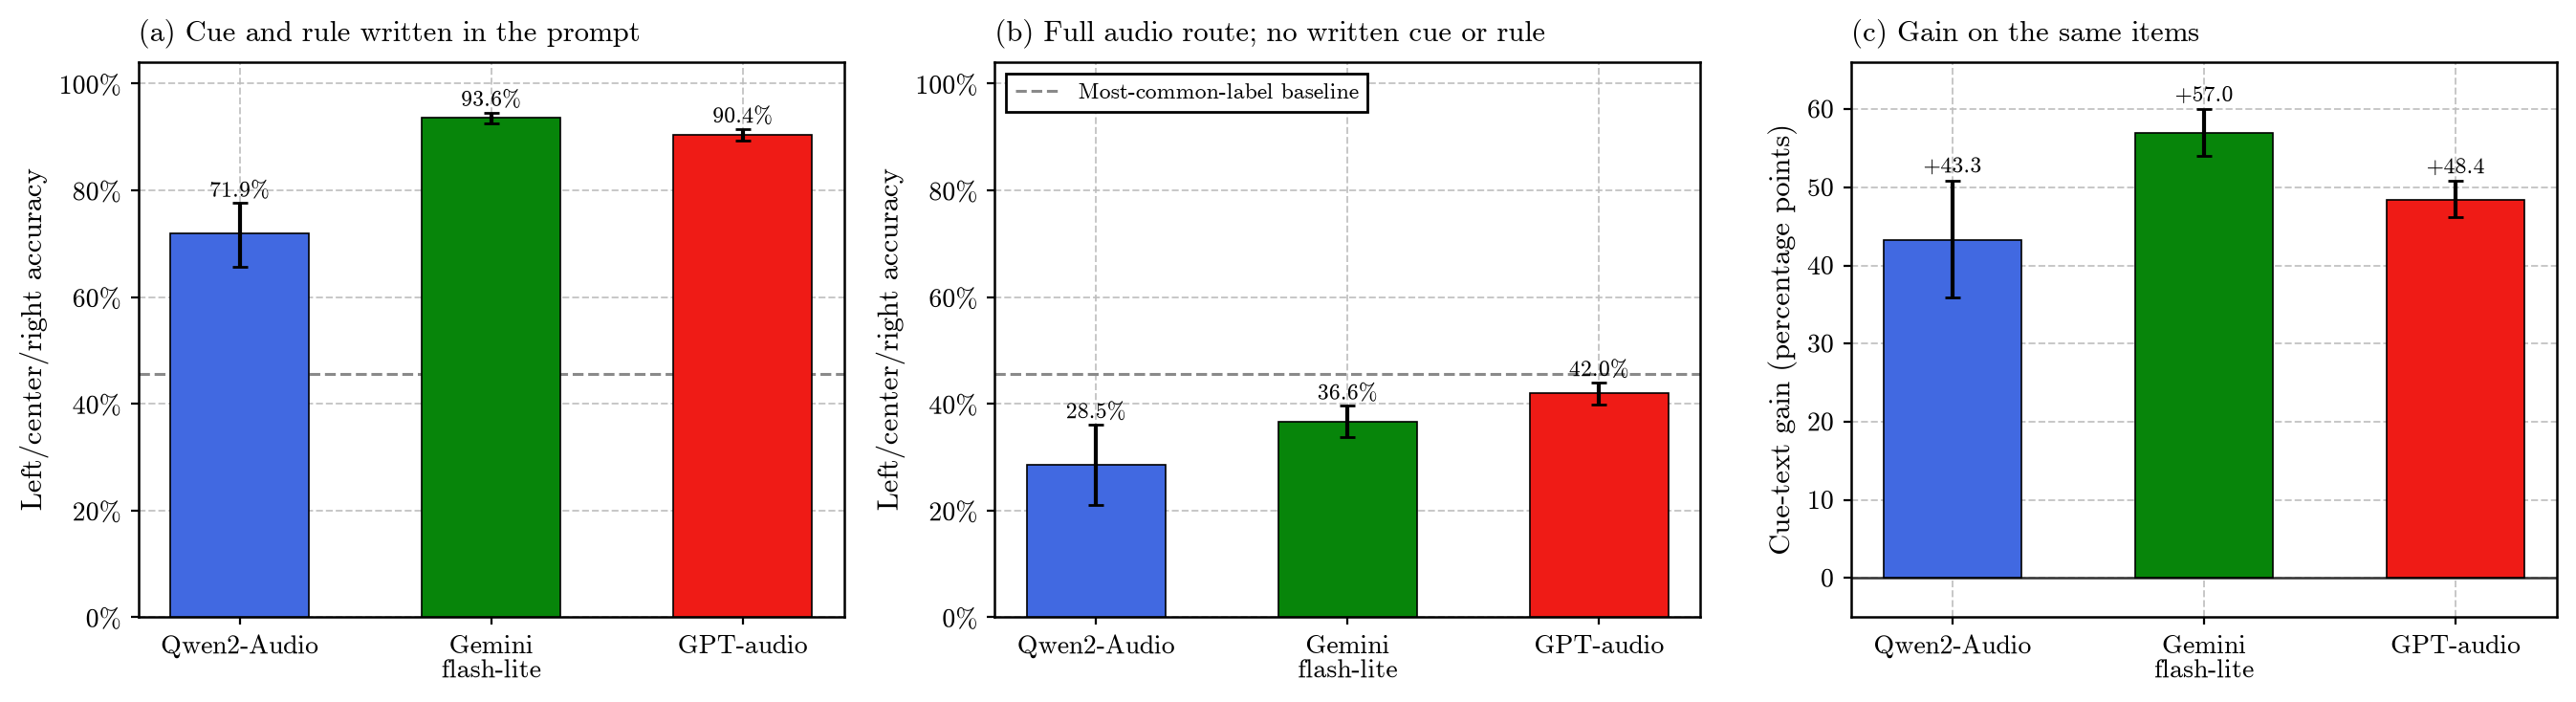
\includegraphics[width=\linewidth]{figures/fig1_reasoning_vs_perception.png}
\caption{The main paired result. Panels (a) and (b) show left/center/right accuracy: the percentage of items assigned the correct one of those three labels. Panel (a) supplies the level cue and conversion rule in text; panel (b) requires the model to obtain and use a relationship from audio. The dashed line marks 45.5\%, the score from always choosing the most common test label. Panel (c) subtracts audio-only accuracy from cue-text accuracy for each model. Error bars are 95\% confidence intervals obtained by resampling the 19 held-out source tracks 20,000 times while keeping each item's two conditions paired.}
\label{fig:main-gap}
\end{figure}

Qwen2-Audio improves from 28.5\% to 71.9\%, Gemini Flash-Lite from 36.6\% to 93.6\%, and GPT-audio from 42.0\% to 90.4\%. These are increases of 43.3, 57.0, and 48.4 percentage points on the same items. Every 95\% interval for the paired increase stays above zero. None of the audio-only estimates, or their intervals, reaches the 45.5\% score of a trivial system that always chooses the most common label.

The errors do not reflect one common physical interpretation. Instead, each model tends to fall back on a preferred answer: Qwen2-Audio often says right, while Gemini and GPT-audio often say left. This pattern is consistent with answer bias rather than reliable use of the channel relationship.

The right label is somewhat more common than center, so raw accuracy can reward a default answer. Table~\ref{tab:complete-results} therefore reports balanced accuracy and macro-F1, which give equal importance to left, center, and right.

Audio-only balanced accuracy stays near 32\% for all three models, close to the 33.3\% expected from equal performance across three classes. The conclusion also survives the stricter analysis that groups tracks by their six musical pieces: the paired intervals remain above zero for all models. Because six pieces are a small number of groups, we treat this as a sensitivity check rather than the main interval.

This result does not mean the audio contains no information, and it does not identify one broken layer. It means that the complete audio route does not make the relevant left-right evidence reliably usable by the answer-generating system, even though the same system performs much better once that evidence and its conversion rule are written explicitly.

\subsection{Correct side predictions do not guarantee accurate angles}

Choosing left or right requires only the sign of the level difference. Calculating an angle requires using its numerical size correctly. Figure~\ref{fig:angle-faithfulness} summarizes this separation; Table~\ref{tab:complete-results} reports the complete metrics.

\begin{figure}[!htbp]
\centering
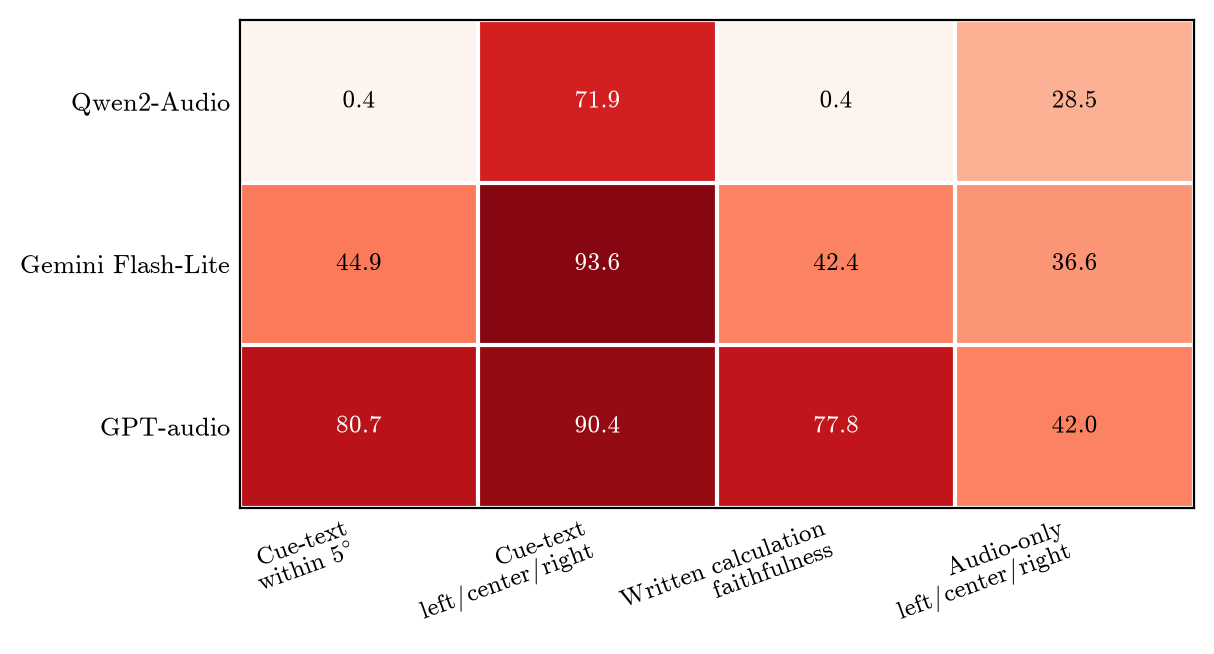
\includegraphics[width=0.92\linewidth]{figures/fig6_model_metric_heatmap.png}
\caption{Correct side does not guarantee an accurate angle or a faithful calculation. Values are percentages on the same 1,045 cue-text items, except the final column, which reports audio-only left/center/right accuracy. Written-calculation faithfulness measures whether the displayed steps follow from the cue stated in the response.}
\label{fig:angle-faithfulness}
\end{figure}

Qwen2-Audio reaches 71.9\% cue-text left/center/right accuracy but only 0.4\% within-\(5^\circ\) angle accuracy. It usually identifies the louder side without carrying out the supplied conversion correctly. Gemini and GPT-audio calculate the angles more successfully, at 44.9\% and 80.7\% within \(5^\circ\), but their written calculations are not always faithful to the stated cue. Premise-grounded verifier faithfulness is 0.4\%, 42.4\%, and 77.8\% for Qwen2-Audio, Gemini, and GPT-audio, respectively.

A common error is \emph{boundary substitution}. The prompt explains that the virtual speakers are at \(-30^\circ\) and \(+30^\circ\). Instead of evaluating the equation for the current item, the model sometimes repeats 30 degrees as if it were the answer. This occurs in nearly every answered Qwen2-Audio item, 19.7\% of Gemini's answered items, and 1.2\% of GPT-audio's.

Qwen2-Audio's mean error can exceed the benchmark's 30-degree limit because we score the angle exactly as generated. We do not silently clip an answer such as 90 degrees back into the allowed range.

Two supporting analyses are reported outside the main results. Appendix~\ref{sec:appendix-offgrid} documents the off-grid fine-tuning audit that motivated premise-grounded verification. Appendix~\ref{sec:appendix-probe} reports a preliminary Qwen2-Audio encoder probe; the probe supplies its own left-right subtraction, so it is not evidence that the complete model performs that comparison.

\section{Discussion}
\label{sec:discussion}

\paragraph{What ECHO establishes.} On the same items and models, performance changes sharply when the cue and rule are written down. This shows a practical difference between best-case explicit cue use and the full audio route; it does not isolate one mental ability or encoder layer. "Cue access" includes channel encoding, comparison, audio--language alignment, answer generation. The distinction still matters because arithmetic training cannot recover a cue that never becomes usable, while better audio processing does not ensure correct calculation.

Cue-text success also has a narrow meaning: the model used explicit information under this prompt, not that it possesses general spatial reasoning. Likewise, our verifier checks whether the visible calculation follows from the stated cue. A convincing derivation can still contain arithmetic that does not follow from the evidence written in its first line.

\paragraph{Case study: locating a failure after the cue.} Consider one held-out off-grid item whose true position is \(21.8^\circ\) to the right and whose measured ILD is \(-14.8\) dB. The fine-tuned Qwen2-Audio response correctly repeats that cue and identifies the right side, but then writes \(r=10^{-14.8/20}=0.139\) and concludes \(-23.6^\circ\). ECHO's verifier recomputes the displayed step and finds that the ratio should be approximately \(0.182\), not \(0.139\). The written value \(0.139\) instead corresponds to a nearby \(-17.2\) dB training cue whose stored answer is \(-23.6^\circ\). This example locates the failure after the premise is available: the model copies the new cue but substitutes a memorized cue during calculation. The same pattern occurs in 189 of 190 original off-grid responses. A final-answer metric alone would report only a \(1.8^\circ\) error; the premise-grounded check reveals the shortcut that produced it.

\paragraph{Implications.} The Qwen probe suggests that jointly comparing channels may be more useful than simply unfreezing an entire encoder. For evaluation, file count is not problem diversity: benchmarks should report distinct cue--answer relationships, test values between training points, and verify each written step from the model's stated premise. Preliminary dithering experiments perturb the failure but collapse to a few answer templates; Appendix~\ref{sec:appendix-dithering} reports them as future-work evidence, not a solution.

\paragraph{Broader impact.} More diagnostic spatial evaluation could improve the reliability of music-production tools, accessibility systems, and other audio assistants by showing whether a failure comes from unavailable evidence or incorrect use of that evidence. The main risk is overgeneralization: success on controlled amplitude panning does not establish reliable localization in rooms, natural binaural hearing, or safety-critical settings. We mitigate this risk by releasing the verifier and benchmark audit, reporting negative results, and limiting our claims to the tested cue, delivery protocol, and model families.

\section{Limitations}
\label{sec:limitations}

While ECHO reveals a consistent operational gap on the tested systems, we note several limitations. The positions use controlled studio panning, not natural hearing. Cue-text provides both the cue and rule, so an audio-plus-rule condition is still needed to separate cue extraction from knowledge of the rule. Left and right are delivered as two labeled clips rather than one native stereo file. The study covers 19 tracks from six pieces and only three model families; the undisclosed sizes of Gemini Flash-Lite and GPT-audio prevent a meaningful analysis of scaling. Hosted systems may also change. The two conditions require different fixed parsing rules, and hosted models are sampled once per item.

\section{Conclusion}

ECHO treats localization as a sequence of steps rather than one final score: audio must contain a cue, the model must make that cue usable, the cue must be converted into an answer, and any written calculation should follow from the evidence provided. StereoMusicQA makes each stage checkable by connecting a real instrument recording, a measured left-right difference, and a known source angle.

Across Qwen2-Audio, Gemini Flash-Lite, and GPT-audio, writing the cue and conversion rule in the prompt improves left/center/right accuracy by 43.3--57.0 percentage points, while audio-only accuracy remains below the score from always choosing the most common label. The models therefore perform substantially better under best-case explicit cue use than through the complete audio route. Exact audio calculation and written-calculation faithfulness remain separate weaknesses. These findings show why spatial evaluation should report where the pipeline fails, not only whether the last answer is correct. More broadly, evaluation can overstate a model's ability whenever it confuses access to evidence with reasoning from that evidence, or mistakes a convincing written derivation for a faithful one.

\bibliographystyle{plainnat}
\bibliography{references}
\appendix
\makeatletter
\@addtoreset{figure}{section}
\@addtoreset{table}{section}
\renewcommand{\thefigure}{\thesection\arabic{figure}}
\renewcommand{\thetable}{\thesection\arabic{table}}
\makeatother

\section{Complete zero-shot results}

Balanced accuracy averages the fraction correctly identified within each of the three position labels. Precision asks how often a predicted label is correct, recall asks how many true items with that label are found, and F1 combines the two. Macro-F1 computes F1 separately for left, center, and right and averages the three. Coverage is the fraction of responses containing an extractable angle.

\begin{table}[H]
\caption{Complete zero-shot results for the three evaluated systems.}
\label{tab:complete-results}
\centering
\setlength{\tabcolsep}{4pt}
\begin{tabular}{>{\raggedright\arraybackslash}p{0.42\linewidth}ccc}
\toprule
Metric & Qwen2-Audio & Gemini Flash-Lite & GPT-audio \\
\midrule
Cue-text within-\(5^\circ\) & 0.4\% & 44.9\% & 80.7\% \\
Cue-text mean absolute angle error & \(74.27^\circ\) & \(7.49^\circ\) & \(5.44^\circ\) \\
Cue-text left/center/right accuracy & 71.9\% & 93.6\% & 90.4\% \\
Cue-text verifier faithfulness & 0.4\% & 42.4\% & 77.8\% \\
Audio-only left/center/right accuracy & 28.5\% & 36.6\% & 42.0\% \\
Cue-text balanced accuracy & 53.0\% & 83.8\% & 82.6\% \\
Audio-only balanced accuracy & 31.9\% & 32.7\% & 31.4\% \\
Cue-text macro-F1 & 51.4\% & 88.7\% & 86.4\% \\
Audio-only macro-F1 & 26.0\% & 31.2\% & 28.0\% \\
Cue-text coverage & 97.6\% & 96.8\% & 99.8\% \\
Boundary-substitution rate among answered items & \(\sim100\%\) &
19.7\% & 1.2\% \\
\bottomrule
\end{tabular}
\end{table}

\begin{table}[H]
\caption{Exact left/center/right results for the two item-matched ECHO conditions. Brackets show 95\% confidence intervals obtained by resampling complete source tracks while preserving each cue text/audio-only pair; pp means percentage points.}
\label{tab:cue-access-gap}
\centering
\setlength{\tabcolsep}{5pt}
\renewcommand{\arraystretch}{1.12}
\begin{tabular}{lccc}
\toprule
Model & Cue-text accuracy & Audio-only accuracy & Paired gap \\
\midrule
Qwen2-Audio &
\parbox[c]{0.20\linewidth}{\centering 71.9\% \\ {[65.6, 77.6]}} &
\parbox[c]{0.20\linewidth}{\centering 28.5\% \\ {[21.0, 36.1]}} &
\parbox[c]{0.18\linewidth}{\centering \textbf{+43.3 pp} \\ {[35.9, 50.9]}} \\
Gemini Flash-Lite &
\parbox[c]{0.20\linewidth}{\centering 93.6\% \\ {[92.5, 94.6]}} &
\parbox[c]{0.20\linewidth}{\centering 36.6\% \\ {[33.7, 39.6]}} &
\parbox[c]{0.18\linewidth}{\centering \textbf{+57.0 pp} \\ {[54.0, 60.0]}} \\
GPT-audio &
\parbox[c]{0.20\linewidth}{\centering 90.4\% \\ {[89.4, 91.5]}} &
\parbox[c]{0.20\linewidth}{\centering 42.0\% \\ {[39.9, 44.0]}} &
\parbox[c]{0.18\linewidth}{\centering \textbf{+48.4 pp} \\ {[46.2, 50.8]}} \\
\bottomrule
\end{tabular}
\end{table}

\begin{figure}[H]
\centering
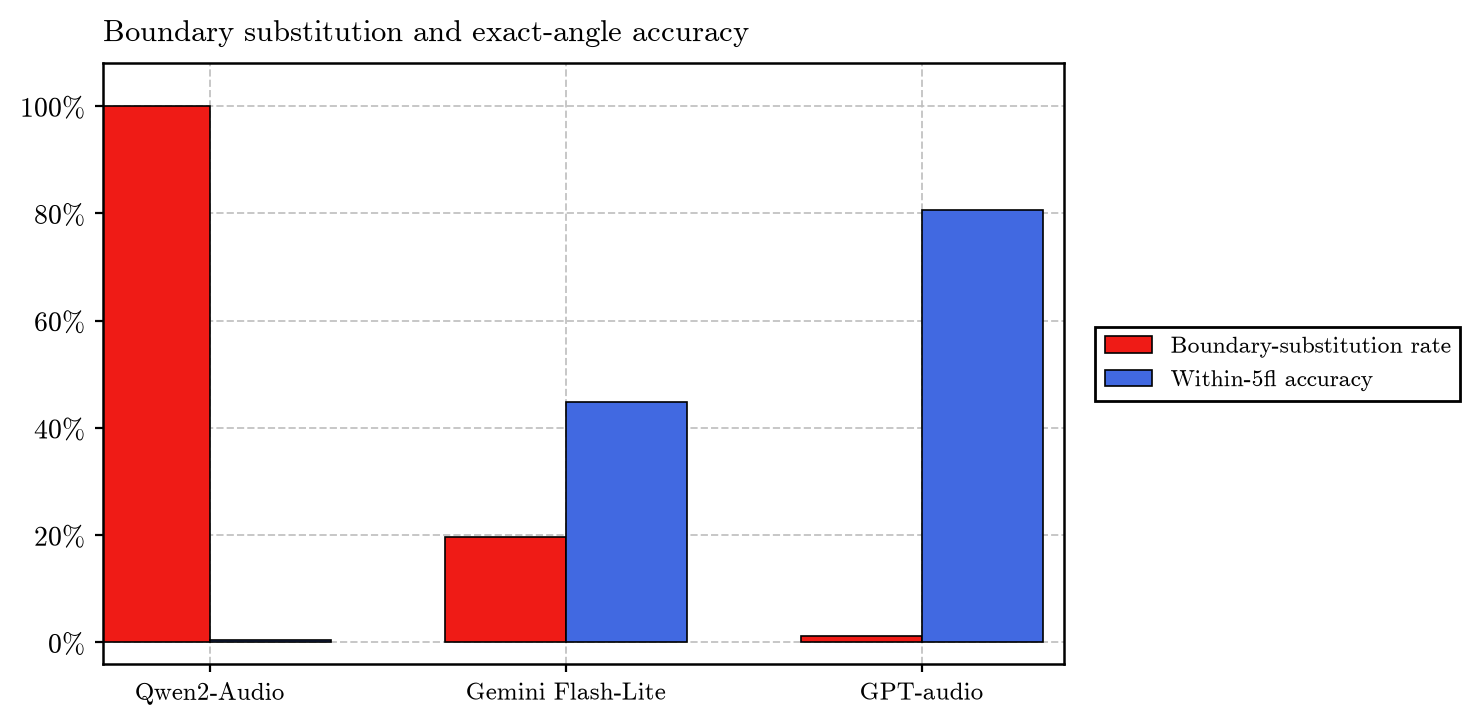
\includegraphics[width=\linewidth]{figures/fig_appendix_boundary_snap.png}
\caption{Descriptive results for the three evaluated systems. Bars are not connected because three model endpoints do not establish a scaling trend.}
\end{figure}

\section{Off-grid audit and bounded repair}
\label{sec:appendix-offgrid}

We originally fine-tuned Qwen2-Audio on cue-text examples. Its within-\(5^\circ\) accuracy increased from 0.4\% to 100\%, but the training and standard test sets displayed the same 21 cue-answer pairs at different recordings. We therefore created 190 off-grid items at ten new angles between the trained values. Every prediction landed on one of the old 21 angles. In 189 of 190 responses, the model first copied the new cue and then calculated with a different value from the training grid. The answer looked like a solved equation, but the arithmetic did not follow from its own premise.

This audit motivated the premise-grounded verifier used in the main study. The original verifier checked intermediate values against stored labels; the corrected version recomputes every displayed step from the cue written in the response. Only 0.5\% of the original off-grid derivations pass that stricter check. This appendix records the failed fine-tuning attempt as a benchmark audit, not as a general claim about audio-language models.

\begin{figure}[H]
\centering
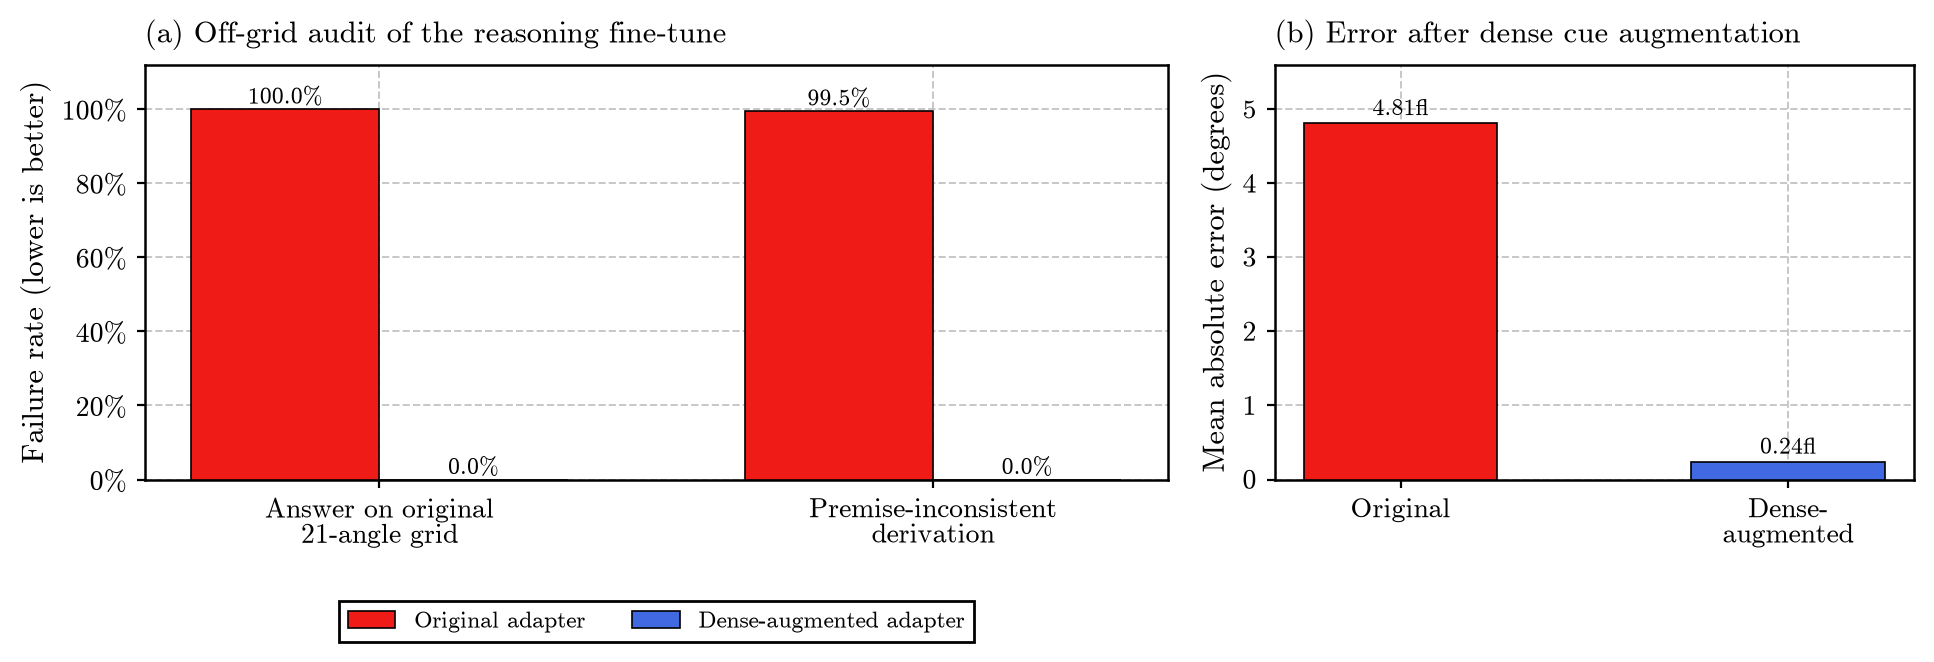
\includegraphics[width=\linewidth]{figures/fig2_lookup_table_before_after.png}
\caption{The original fine-tuned model's off-grid outputs expose the 21-row lookup. ``Off-grid'' means that the test cue lies between values used during training. Every answer lands on the old training grid, and 99.5\% contain arithmetic that does not follow from the cue stated in the response. Adding many intermediate cue values to training removes those specific indicators and reduces mean absolute error (MAE) from \(4.81^\circ\) to \(0.24^\circ\).}
\end{figure}

The dense-augmentation run adds 3,000 continuously sampled cue-answer examples, producing 606 displayed ILDs and 430 displayed azimuths. The ten off-grid test angles are excluded during sampling. On the original 1,045-item test set, the fine-tuned model retains 100\% within-\(5^\circ\) accuracy and reaches 100\% premise-grounded faithfulness. On the 190 off-grid items, it reaches 100\% within-\(5^\circ\), \(0.24^\circ\) MAE, and 100\% verifier faithfulness.

These results eliminate the specific 21-row failure. They do not prove that the model executes the symbolic law. All 190 repaired predictions fall within \(0.2^\circ\) of some dense training azimuth, so accurate interpolation remains a complete alternative explanation. The repair is therefore reported as benchmark hardening, not as proof of human-like computation.

\section{Preliminary dithering experiment}
\label{sec:appendix-dithering}

\begin{figure}[H]
\centering
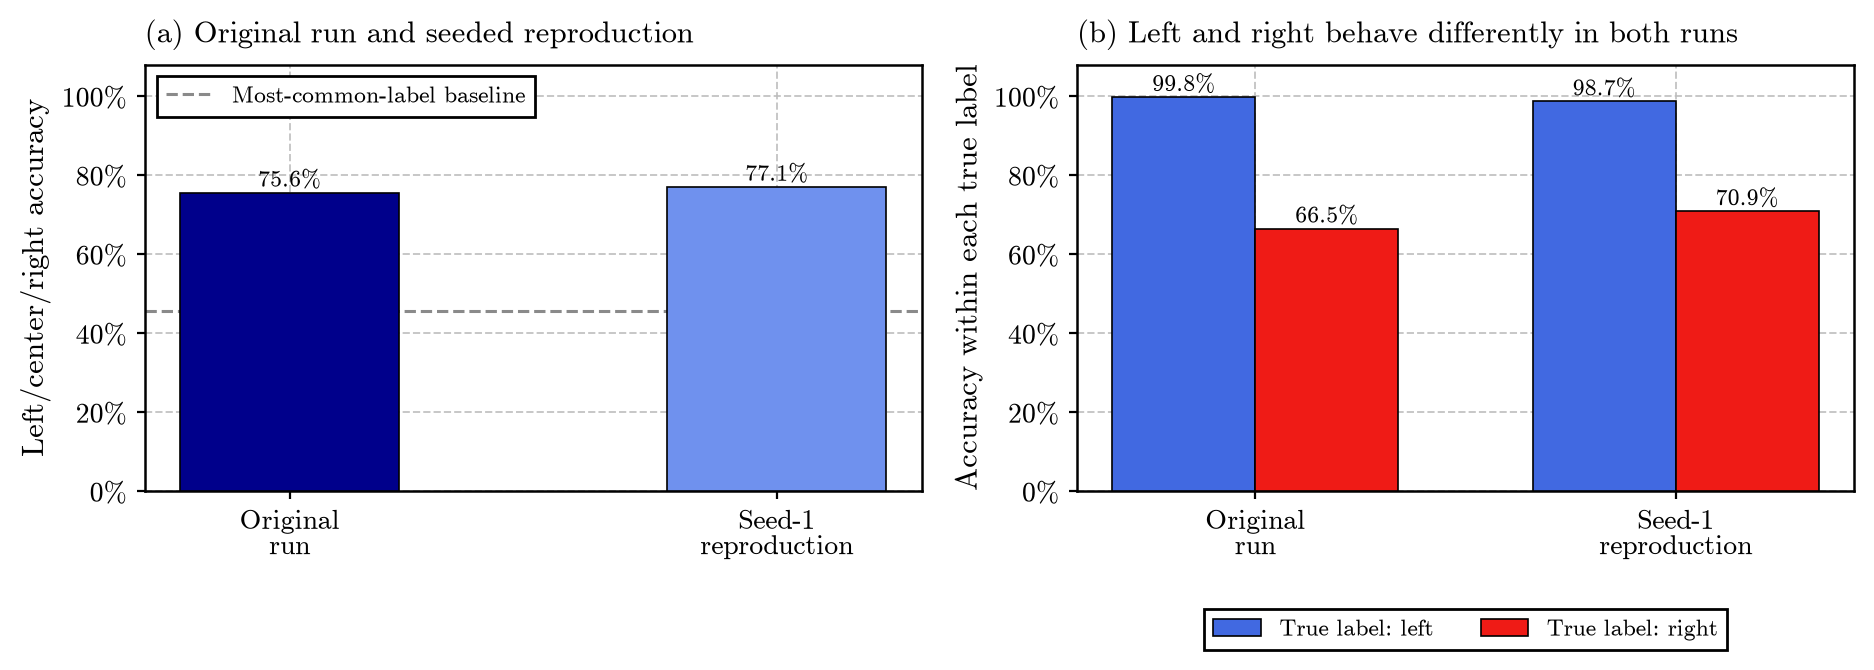
\includegraphics[width=\linewidth]{figures/fig3_dithering_replication.png}
\caption{Training-time dithering---adding small random noise to each audio channel during training---raises Qwen2-Audio left/center/right accuracy to 75.6\% in the original run and 77.1\% in a reproduction with training-noise seed 1. Both fine-tuned models are evaluated with the same noise sequence, identified by seed 101. The output remains severely template-collapsed: it reuses only a few answer patterns and never identifies the center correctly.}
\end{figure}

\begin{table}[H]
\caption{Left/center/right accuracy for the original dithering run and its seeded reproduction.}
\label{tab:dithering-reproduction}
\centering
\begin{tabular}{lrr}
\toprule
Metric & Original run & Seed-1 reproduction \\
\midrule
Left/center/right accuracy & 75.6\% & 77.1\% \\
True-left correct & 99.8\% & 98.7\% \\
True-right correct & 66.5\% & 70.9\% \\
True-center correct & 0.0\% & 0.0\% \\
\bottomrule
\end{tabular}
\end{table}

Inference-only dithering does not produce a reliable gain. Training-time dithering does, but the model emits only a few fixed sentence templates and does not recover exact localization. Fully unfreezing the encoder regresses to 45.5\% after one epoch and 46.4\% after three epochs, both explained by answer collapse rather than true discrimination. These experiments motivate future work on joint channel representations or the audio-language projector.

\begin{figure}[H]
\centering
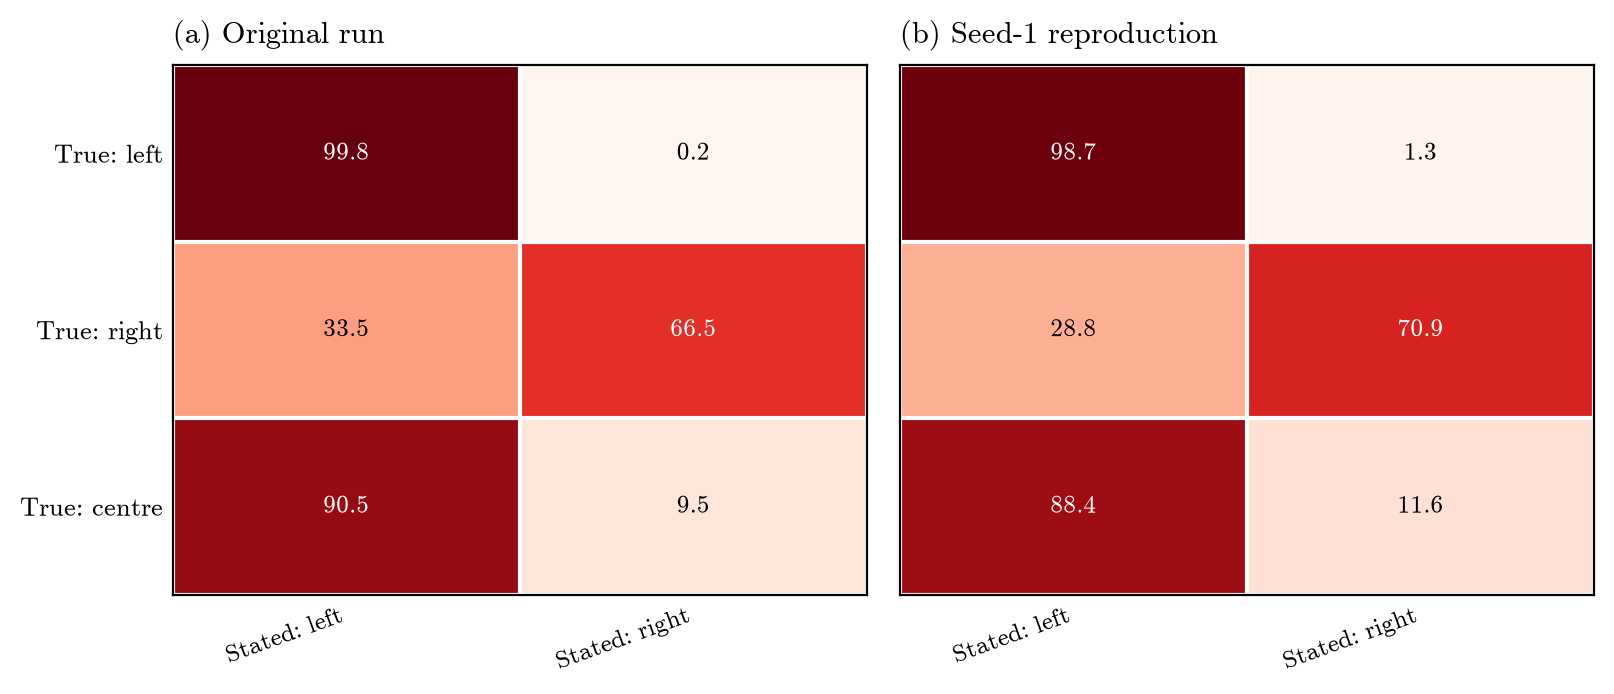
\includegraphics[width=\linewidth]{figures/fig7_dithering_confusion_heatmap.png}
\caption{Dithering confusion matrices. Each row is the true position label, and each column is the label predicted by the model.}
\end{figure}

\section{Reproducibility notes}
\label{sec:appendix-repro}

\subsection{Benchmark construction}
\label{sec:appendix-construction}

We sort the 44 URMP piece identifiers and shuffle them once with Python's Mersenne Twister using seed 2026. A 70/15/15 piece-level split produces 31 training pieces, seven development pieces, and six test pieces; no isolated source track (or \emph{stem}) from a piece crosses splits. The inventory contains 149 mono instrument stems. For each stem at least six seconds long, we derive a stem-specific 64-bit seed from the first eight bytes of SHA-256(``2026:'') and use that seed to draw one uniform six-second excerpt offset. The same excerpt is reused for all angles and processing conditions, so comparisons do not confound position with musical content.

Each excerpt is resampled to 48 kHz (48,000 audio samples per second) and rendered at \(-25^\circ\),
\(-20^\circ\), \(-15^\circ\), \(-10^\circ\), \(-5^\circ\),
\(0^\circ\), \(5^\circ\), \(10^\circ\), \(15^\circ\),
\(20^\circ\), and \(25^\circ\). The dry render, meaning no additional processing, uses the tangent amplitude-panning rule with virtual speakers at \(\pm 30^\circ\). Four additional renders apply one transformation after panning: 4:1 dynamic-range compression above \(-20\) dB, a +6 dB equalizer that changes frequency balance around 1 kHz, stereo widening that separately scales the shared and differing parts of the two channels (mid/side widening) with width 1.2, or a 300 microsecond delay on the right channel. This gives 8,195 candidate renders. A candidate is rejected if it is non-stereo, contains invalid numerical samples, is quieter than \(-45\) dB root-mean-square (RMS) level---a measure of average signal level---has peaks above 0.99, or fails to recover the processing-adjusted azimuth within \(5^\circ\). We additionally require the expected inter-channel delay within 30 microseconds, the expected regime label, and channel coherence---a measure of similarity between the two channel waveforms---of at least 0.90 whenever the processing should preserve a narrow spatial source. These checks retain 7,718 items: 5,332 training, 1,341 development, and 1,045 test items. Audio is stored as 24-bit pulse-code modulated (PCM) WAV files, a standard uncompressed digital-audio format; public test identifiers conceal stem, offset, and angle, while those fields are retained in the private labels.

\subsection{Zero-shot inference}
\label{sec:appendix-zero-shot}

Every model receives the same held-out items and one completion per condition; we do not ask the same question several times and vote among the answers, a procedure often called self-consistency sampling. For cue-text evaluation, ILD is measured on the 48 kHz render before the audio is downmixed to mono, and the prompt supplies that measurement and the panning law. For audio-only evaluation, the left and right waveforms are supplied as separately identified audio inputs and the prompt contains no measured cue. Qwen2-Audio resamples each input independently to 16 kHz, uses the bfloat16 numerical format, and always selects its highest-scoring next token (greedy decoding) with a limit of 200 new tokens. Gemini Flash-Lite and GPT-audio receive 48 kHz 16-bit PCM WAV data through their provider APIs. Those hosted calls used the providers' default generation settings, which did not expose a fixed seed in our evaluation path. Their reported values are therefore one-answer measurements of those hosted service versions, not estimates averaged over repeated random seeds. Failed API calls were retried up to three times; completed item identifiers were checkpointed so a resumed run did not generate a second answer for an already completed item.

\subsection{Statistical analysis}
\label{sec:appendix-stats}

The headline confidence intervals use the paired cluster bootstrap described in Section~\ref{sec:uncertainty}: 20,000 resamples of the 19 complete held-out stem clusters with replacement, seed 20,260,814, and percentile endpoints at 2.5\% and 97.5\%. Pairing is preserved both across conditions and across all transformations of a stem. No item-level independence assumption is used, and no correction for multiple comparisons is applied. The majority baseline is deterministic: it always predicts right, one of two tied most-frequent test labels, and is correct for 475/1,045 items (45.5\%); always-left has the same accuracy.

As a stricter dependence sensitivity analysis, we repeat the paired bootstrap while clustering by the six held-out URMP pieces. The paired-gap intervals are {[}37.3, 50.2{]}, {[}55.5, 59.4{]}, and {[}46.3, 50.5{]} percentage points for Qwen2-Audio, Gemini Flash-Lite, and GPT-audio, respectively. All exclude zero, but the small number of piece clusters makes these intervals secondary to the stem-cluster analysis. We also compute balanced accuracy and macro-F1 directly from the three-class confusion matrices; these are point estimates, not additional hypothesis tests.

\subsection{Qwen2-Audio fine-tuning and off-grid audit}
\label{sec:appendix-finetuning}

All Qwen fine-tunes use quantized low-rank adaptation (QLoRA), which trains small added weight matrices while keeping the 4-bit NormalFloat (NF4)-quantized base model fixed. Computation uses bfloat16 and gradient checkpointing, which saves memory by recomputing some intermediate values, QLoRA rank 16, scale 32, and dropout 0.05, meaning that 5\% of the adapter's units are randomly disabled during each training step. AdamW uses a learning rate of \(2 \times 10^{-4}\), one example per forward pass, and eight-step gradient accumulation, meaning that eight examples contribute before each weight update. Unless an experiment states otherwise, training makes one pass over the 5,332 training items. Prompt tokens are masked, so the loss is applied only to the target answer. The original suffix-based LoRA target list adapts the language model's query, key, value, output, gate, up, and down projections; because Qwen2-Audio reuses the query/key/value names in its audio tower, it also adapts those three projections in all 32 encoder layers. The audio-to-language projector, which connects audio features to the language model, and the remaining encoder weights stay frozen in that configuration.

The dense repair appends 3,000 cue-answer pairs generated with seed 2026. Azimuths are sampled uniformly from \([-29.5^\circ, 29.5^\circ]\), rejecting values within \(0.2^\circ\) of any of the ten off-grid evaluation angles. Each sampled azimuth is converted to ILD by the exact inverse panning law, and its target derivation is computed forward from the displayed cue. These examples reuse real training audio only as the required audio placeholder; the cue-text condition is deliberately solved from the supplied symbolic cue. The repaired QLoRA adapter is trained for one pass over 5,332 real plus 3,000 synthetic examples and is evaluated both on the original 1,045 items and on 190 items constructed at ten withheld angles: \(\pm2.5^\circ\), \(\pm8.0^\circ\), \(\pm13.5^\circ\),
\(\pm16.4^\circ\), and \(\pm21.8^\circ\).

Not every training source of randomness was fixed in the historical runs. The original reasoning adapter and dense-repair adapter are single optimization runs without an explicitly recorded PyTorch/CUDA seed. Likewise, the first dithering run drew training noise from an unseeded generator. The dithering reproduction fixes training-noise and Torch seed 1; both the original and reproduced adapters are then evaluated on the same independent Gaussian noise sequence with seed 101. Dithering adds independent Gaussian noise drawn from the standard normal distribution, \(N(0,1)\), to every sample of each channel at amplitude 0.05. Thus the 75.6\%/77.1\% agreement is a seeded
reproduction of the intervention's qualitative effect, but the other fine-tune numbers should not be presented as multi-seed means.

\subsection{Encoder probe and verifier audit}
\label{sec:appendix-probe}

\begin{figure}[H]
\centering
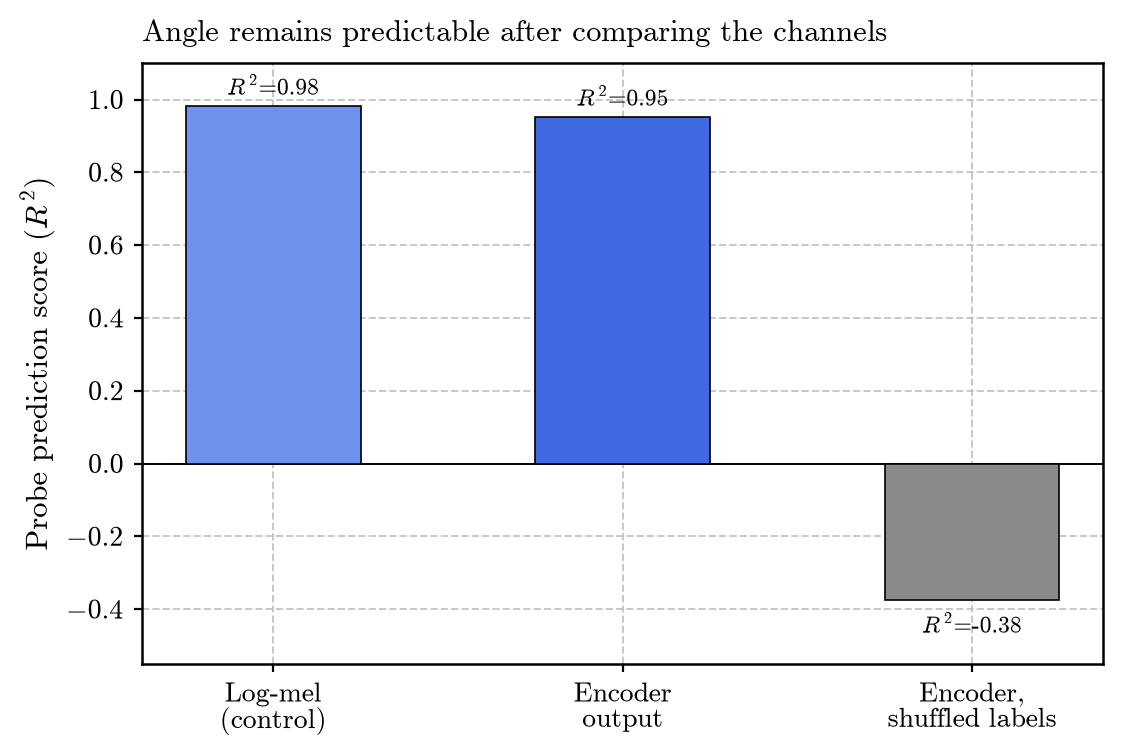
\includegraphics[width=0.82\linewidth]{figures/fig_appendix_encoder_probe.png}
\caption{A simple diagnostic predictor recovers source angle when we explicitly subtract right-channel features from left-channel features. Prediction reaches \(R^2=0.98\) from standard log-mel features and \(R^2=0.95\) from frozen Qwen2-Audio encoder features. An \(R^2\) near 1 indicates strong prediction. Shuffling the angle labels provides a negative control and produces \(R^2=-0.38\).}
\label{fig:encoder-probe}
\end{figure}

The encoder probe uses seed 2026. From the held-out split, it selects ten six-second excerpts; for each selected stem it draws 20 candidate offsets and keeps the one with the highest RMS. Each excerpt is rendered at the eleven main benchmark angles, producing 110 observations. Left and right channels are encoded separately, feature vectors from valid time frames are averaged (mean-pooled), and the right feature vector is subtracted from the left. A ridge regressor---
a linear model with an \(L_2\) penalty---is evaluated by leave-one-excerpt-out cross-validation. The procedure repeatedly trains on nine excerpts and tests on the remaining one, so all eleven angles from the test excerpt are excluded from its training fold. The shuffled control permutes angle labels within each excerpt
with seed 2027 while preserving features, groups, and fold sizes.

During the off-grid audit, we found that the original verifier compared claims with stored ground truth but did not recompute an intermediate value from the premise written in the model's own derivation. The corrected verifier parses expressions of the form \(r = 10^{x/20} = y\) and checks \(y\) against the stated \(x\) before checking the final angle. We also found that an earlier target generator displayed ILD rounded to one decimal while computing an intermediate value from the unrounded ILD. The discrepancy was at most 0.05 dB and did not alter a reported aggregate, but all current targets compute downstream quantities from the displayed premise. Benchmark manifests, prompts, raw model completions, private scoring labels, rejection records, and experiment configurations are available in the \href{https://anonymous.4open.science/r/ECHO-FC6D/}{anonymous artifact repository}; URMP source audio must be obtained from its original distribution.

\section{Design comparison with related benchmarks}

\begin{table}[H]
\caption{Design comparison with adjacent physical-audio and spatial-audio resources. The table distinguishes evaluation benchmarks from systems that introduce specialized spatial training.}
\label{tab:benchmark-comparison}
\centering
\footnotesize
\setlength{\tabcolsep}{3pt}
\renewcommand{\arraystretch}{1.35}
\begin{tabular}{
>{\raggedright\arraybackslash}p{0.13\linewidth}
>{\raggedright\arraybackslash}p{0.16\linewidth}
>{\raggedright\arraybackslash}p{0.22\linewidth}
>{\raggedright\arraybackslash}p{0.19\linewidth}
>{\raggedright\arraybackslash}p{0.19\linewidth}}
\toprule
Resource & Primary question & Spatial evidence and labels & Experimental contrast & Audit \\
\midrule
AV-Odyssey \citep{gong2024avodyssey} & Can multimodal models combine audio and visual clues, including basic loudness and pitch? & Carefully constructed audio-visual multiple-choice problems; not a spatial-localization benchmark & Audio-visual reasoning across 4,555 problems & Objective choices; a matched spatial cue intervention is not reported \\ SonicBench \citep{sun2026sonicbench} & How broadly do models perceive physical audio attributes? & Controlled stimuli for 12 attributes; direction uses coarse front-versus-back sectors & Recognition versus comparison across 2,400 items & Human and random baselines plus encoder probes; a matched explicit-cue/audio comparison is not reported \\ SpatialSoundQA / BAT \citep{zheng2024bat} & Can a purpose-built model perceive and reason about binaural scenes? & AudioSet sources rendered with SoundSpaces 2.0; localization, distance, and spatial-relation QA & Specialized Spatial-AST--LLM training versus prior systems & Evaluates spatial QA performance; a premise-grounded arithmetic verifier is not reported \\ BiDepth / OWL \citep{biswas2025owl} & Can geometric supervision improve direction, distance, and spatial reasoning? & Binaural audio paired during training with panoramic depth and room impulse responses; o'clock-level azimuth and direction-of-arrival (DoA) labels & Geometry-aware SAGE/OWL versus BAT on BiDepth and SpatialSoundQA & Spatially grounded step-by-step reasoning supervision; matched cue-access and off-grid arithmetic audits are not reported \\ StereoMusicQA / ECHO (ours) & Can a model use a spatial cue that it fails to access through audio? & Real URMP stems rendered at invertible planted horizontal angles; left/center/right label, continuous angle, and recomputable ILD & The same item under explicit cue-text versus audio-only access & Premise-grounded derivation verification and withheld off-grid cues \\
\bottomrule
\end{tabular}
\end{table}

\end{document}
